\documentclass[main.tex]{subfiles}
\begin{document}

\chapter{Implementation}
To ensure a uniform comparison of the algorithms selected in the concept, the external circumstances
must be identical for each algorithm. This chapter will detail the implementation thereof.

\section{System Setup}
It is necessary to perform all experiments on the same machine to ensure a consistent comparison.
We implement all algorithms and further architecture on a Lenovo IdeaPad 5 Pro,
which runs Linux Ubuntu 20.04.5. The laptop has an AMD Ryzen 7 5800H CPU and 16 GB of RAM.

We install the most recent ROS distribution, \textit{ROS Noetic Ninjemys}, as well as \textit{realsense-ros} with all additional dependencies.

% FIXME I think those footnotes with links were a bad idea

\section{Plane Detection Algorithms}
We implement RSPD and OPS using their respective open source implementations on GitHub\footnote{\href{https://github.com/abnerrjo/PlaneDetection}{{https://github.com/abnerrjo/PlaneDetection}}}
\footnote{\href{https://github.com/victor-amblard/OrientedPointSampling}{https://github.com/victor-amblard/OrientedPointSampling}}. Note that, while the implementation of RSPD is provided by the author,
we could not determine whether the user who uploaded his implementation of OPS is affiliated with \citeauthor{Sun_Mordohai_2019}.
Both methods are implemented in C++ and depend on the C++ linear algebra library \textit{Eigen}\footnote{\href{https://eigen.tuxfamily.org/index.php}{https://eigen.tuxfamily.org/index.php}}
and the C++ API of the  Point-Cloud Library\footnote{\href{https://pointclouds.org/}{https://pointclouds.org/}}, \textit{libpcl-dev}.

The authors of 3D-KHT, provide an implementation, in form of a Visual Studio project, on their website \footnote{\href{https://www.inf.ufrgs.br/~oliveira/pubs_files/HT3D/HT3D_page.html}
    {https://www.inf.ufrgs.br/~oliveira/pubs\_files/HT3D/HT3D\_page.html}}. Since the laptop we use does not run Windows, we use \textit{cmake-converter}
\footnote{\href{https://cmakeconverter.readthedocs.io/en/latest/use.html}{https://cmakeconverter.readthedocs.io/}} to convert
the solution to a cmake project we can build using \textit{make}.

\subsection*{OBRG}
To our knowledge, no open-source implementation is available for the algorithm.
We therefore use our own implementation.

Wir schreiben den algorithmus in python. Wir hatten in betracht gezogen, vorgefertigte octree implementierungen zb von 
open3d zu benutzen, aber diese haben uns im endeffekt nicht genug freiraum geboten. Daher implementieren wir unseren eigenen 
octree für die räumliche aufteilung der punktwolke.
Wir teilen, wie in \ref{sec:bg-obrg} beschrieben, einen octree knoten so lange in 8 gleichgroße kinder auf, bis ein predefined
maximum erreicht ist oder die anzahl der included punkte kleiner als ein schwellwert ist.
% FIXME globale liste ist echt langsam: O(|leafs|) vs O(log_8)
% Dazu speichern wir alle blattknoten in einer globalen liste um 
Um die saliency features der leaf nodes zu berechnen, speziell für die normal vektoren, benutzen wir die 
open3d normal estimation.
wir folgen dem pseudocode wie angegeben, mit der ausnahme, dass wir das hinzufügen in eine region angepasst haben.
Da das wort "insert" raum für interpretation lässt, haben wir eine zweite liste geführt, die angibt, ob ein leaf schon
benutzt wurde. Wenn ja, wird die region gesucht, bei dem das leaf schon benutzt wurde, anstatt eine neue region zu erstellen.
Dieser Schritt kompliziert zwar das region growing ein wenig, reduziert jedoch die totale laufzeit des algorithmus, da 
keine redundante regionen mehr vorkommen können.
Da die residual threshold, angular threshold und dmin des papers nicht genauer spezifiziert wurden, waren wir gezwungen
empirisch zu bestimmen, welche werte gut funktionieren:
\begin{itemize}
    \item res th = 0.1 
    \item ang difference = 0.3
    \item d min =  0.1
\end{itemize}

in deren paper wurde auch ein planarity level von 0.7 -0.9 vorgeschlagen, wir nehmen einfach pauschal 0.8.
oder wir führen tests analog zu 3dkht durch, kann auch sein.

zu guter letzt mussten wir uns das general refinement übelst aus dem ärmel leiern, scheint aber größtenteils 
zu funzen. GR betrifft sowieso scheinbar nur die stellen, wo zwei ebenen aufeinander treffen würden, bzw winkel.

Uns ist bewusst dass python eher weniger echtzeitfähig ist, aber die optimierung eines spezifischen algorithmuses 
steht nciht im vordergrund dieser arbeit und würde dementsprechend zu future work gehören.

\section{Dataset / Ground Truth}
Da der benutzte Datensatz den fokus auf semantische segmentierung legt und nicht auf ebenen findung, 
legen wir unsere eigene ground truth an. Dafür benutzen wir cloudcompare. 
Da wir ausserdem nicht pauschal davon ausgehen können, dass "wände" immer planar sind, oder dass drei tische 
immer verschiedene ebene sind (also zusammenstehen, eine ebene formend, aber dennoch verschiedene tische sind) 
sind wir gezwungen jede punktwolke manuell anzusehen und zu editieren. 
% FIXME Zeit?
% TODO beispielbild

\begin{figure} [!ht]
	\centering
	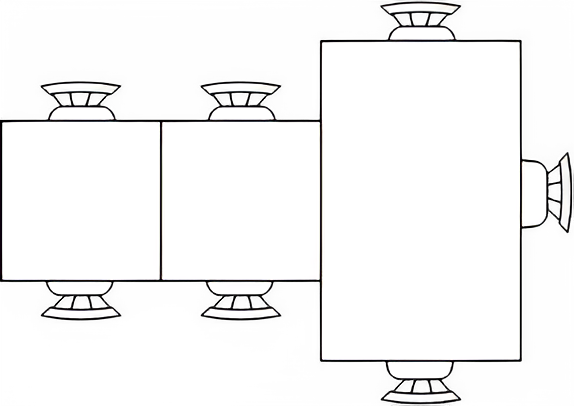
\includegraphics[width=10 cm]{images/tables.png}
	\label{fig:tables}
    \caption{Three tables = three planes?}
\end{figure}


\end{document}



% FIXME section, wie datensätze angelegt werden/wurden
% meilensteine: Tag, wann algos fertig sind
% V1 (ggf aufteilen nach kapitel)

